\documentclass[border=6pt]{standalone}
\usepackage{tikz}
\begin{document}
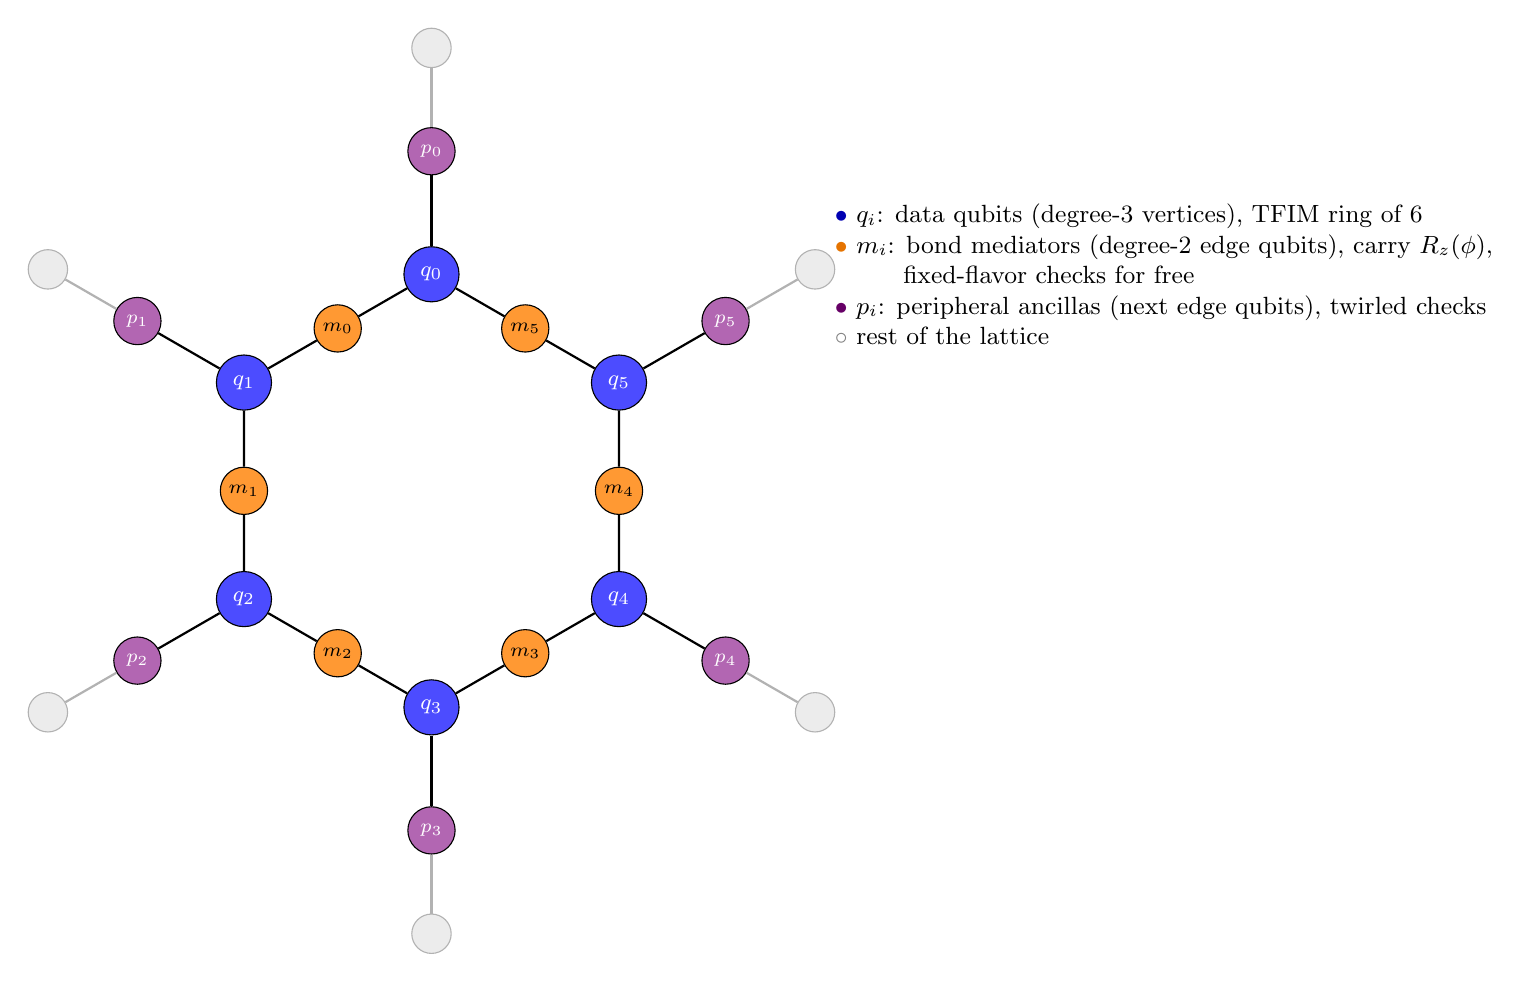
\begin{tikzpicture}[scale=1.25,
  data/.style={circle,draw=black,fill=blue!70,minimum size=7mm,inner sep=0,font=\footnotesize\bfseries,text=white},
  med/.style={circle,draw=black,fill=orange!80,minimum size=6mm,inner sep=0,font=\scriptsize},
  per/.style={circle,draw=black,fill=violet!60,minimum size=6mm,inner sep=0,font=\scriptsize,text=white},
  ghost/.style={circle,draw=gray!60,fill=gray!15,minimum size=5mm,inner sep=0},
  edge/.style={thick}, gedge/.style={gray!60,thick}]
% hexagon of radius R: vertices at 90+60k degrees
\def\R{2.2}
\foreach \k in {0,...,5}{
  \pgfmathsetmacro{\ang}{90+60*\k}
  \pgfmathsetmacro{\angn}{90+60*(\k+1)}
  \pgfmathsetmacro{\angm}{90+60*\k+30}
  % data vertex
  \node[data] (q\k) at (\ang:\R) {$q_{\k}$};
  % mediator at edge midpoint (midpoint of chord: radius R cos30)
  \node[med] (m\k) at (\angm:{\R*cos(30)}) {$m_{\k}$};
  % peripheral ancilla outward
  \node[per] (p\k) at (\ang:{\R+1.25}) {$p_{\k}$};
  % ghost continuation of the lattice beyond the peripheral qubit
  \node[ghost] (g\k) at (\ang:{\R+2.3}) {};
}
\foreach \k [evaluate=\k as \kn using {int(mod(\k+1,6))}] in {0,...,5}{
  \draw[edge] (q\k) -- (m\k) -- (q\kn);
  \draw[edge] (q\k) -- (p\k);
  \draw[gedge] (p\k) -- (g\k);
}
\node[anchor=west,font=\small,align=left] at (4.0,2.2) {%
  \textcolor{blue!70!black}{$\bullet$} $q_i$: data qubits (degree-3 vertices), TFIM ring of 6\\
  \textcolor{orange!90!black}{$\bullet$} $m_i$: bond mediators (degree-2 edge qubits), carry $R_z(\phi)$,\\ \phantom{$\bullet$ $m_i$:} fixed-flavor checks for free\\
  \textcolor{violet!80!black}{$\bullet$} $p_i$: peripheral ancillas (next edge qubits), twirled checks\\
  \textcolor{gray}{$\circ$} rest of the lattice};
\end{tikzpicture}
\end{document}
